\section{Deep Reinforcement Learning Architecture} % 1 page 
%\label{sec:DRLA}
DQN and PG are used in the implemented architecture.
DQN can take advantage of optimal substructures during training. It can also alleviate the impact of long compilation (environment step) time by greatly reducing the data needed. Wang \textit{et al.}~\cite{wang2018} proposed to convert a program into an observation by extracting all the features of the program, \textit{i.e.} number of every operation. Similarly, we extracted program features from the programs. %as listed in Table \ref{tab:tab1}\JENNY{TODO include appendix or not?}\TODO{Ameer: I think so} in the appendix.

Another approach is to use the actions (passes) themselves as observations. In other words, the input of the network (observation) was defined as a histogram of the passes given so far and the passes were given an index from zero to the number of passes. The output is the next pass to apply. This allows the network to keep track of passes applied so far and learn which sequences should be applied to maximize the reward.

We also considered various initial transformations on the programs before running a learning algorithm. We added seven prepasses that will invoke necessary program analysis passes for all programs. This approach reduces the difficulty for the network in finding the best initialization passes. The reward was defined as the negative number of cycles, and thus a higher reward means a lower number of cycles to run the program.

\subsection{Program Features Versus Histogram of Actions}
To evaluate the two approaches, we ran the framework on 12 HLS benchmarks. We trained each benchmark for $30$ minutes. The methodology is described in Section~\ref{sec:results}. Figure~\ref{fig:model-action} shows the circuit speedup as function of time for the two approaches with DQN as the RL algorithm, and -O3, normalized to the performance without any optimization. Both approaches achieve similar performance. The average performance improvement is $13.3\%$ over -O3 and $50\%$ over the performance without any optimization. These improvements are mainly due to the fact that DQN efficiently and robustly learns which passes are useful and which are not.

Figure~\ref{fig:gsm_model_action} shows the mean cycles as a function of time when running the framework on one of the programs (gsm) using the two approaches. Both approaches improve the program's mean cycles over time. We observe two things: (1) Rather than having a smooth line, the instability and chaotic behavior of DQN is seen in the jumps of mean cycles of both approaches. (2) The DQN approach that uses previous passes as the input observation is more stable than using the program features.

\begin{figure}[!t]
    \centering        
    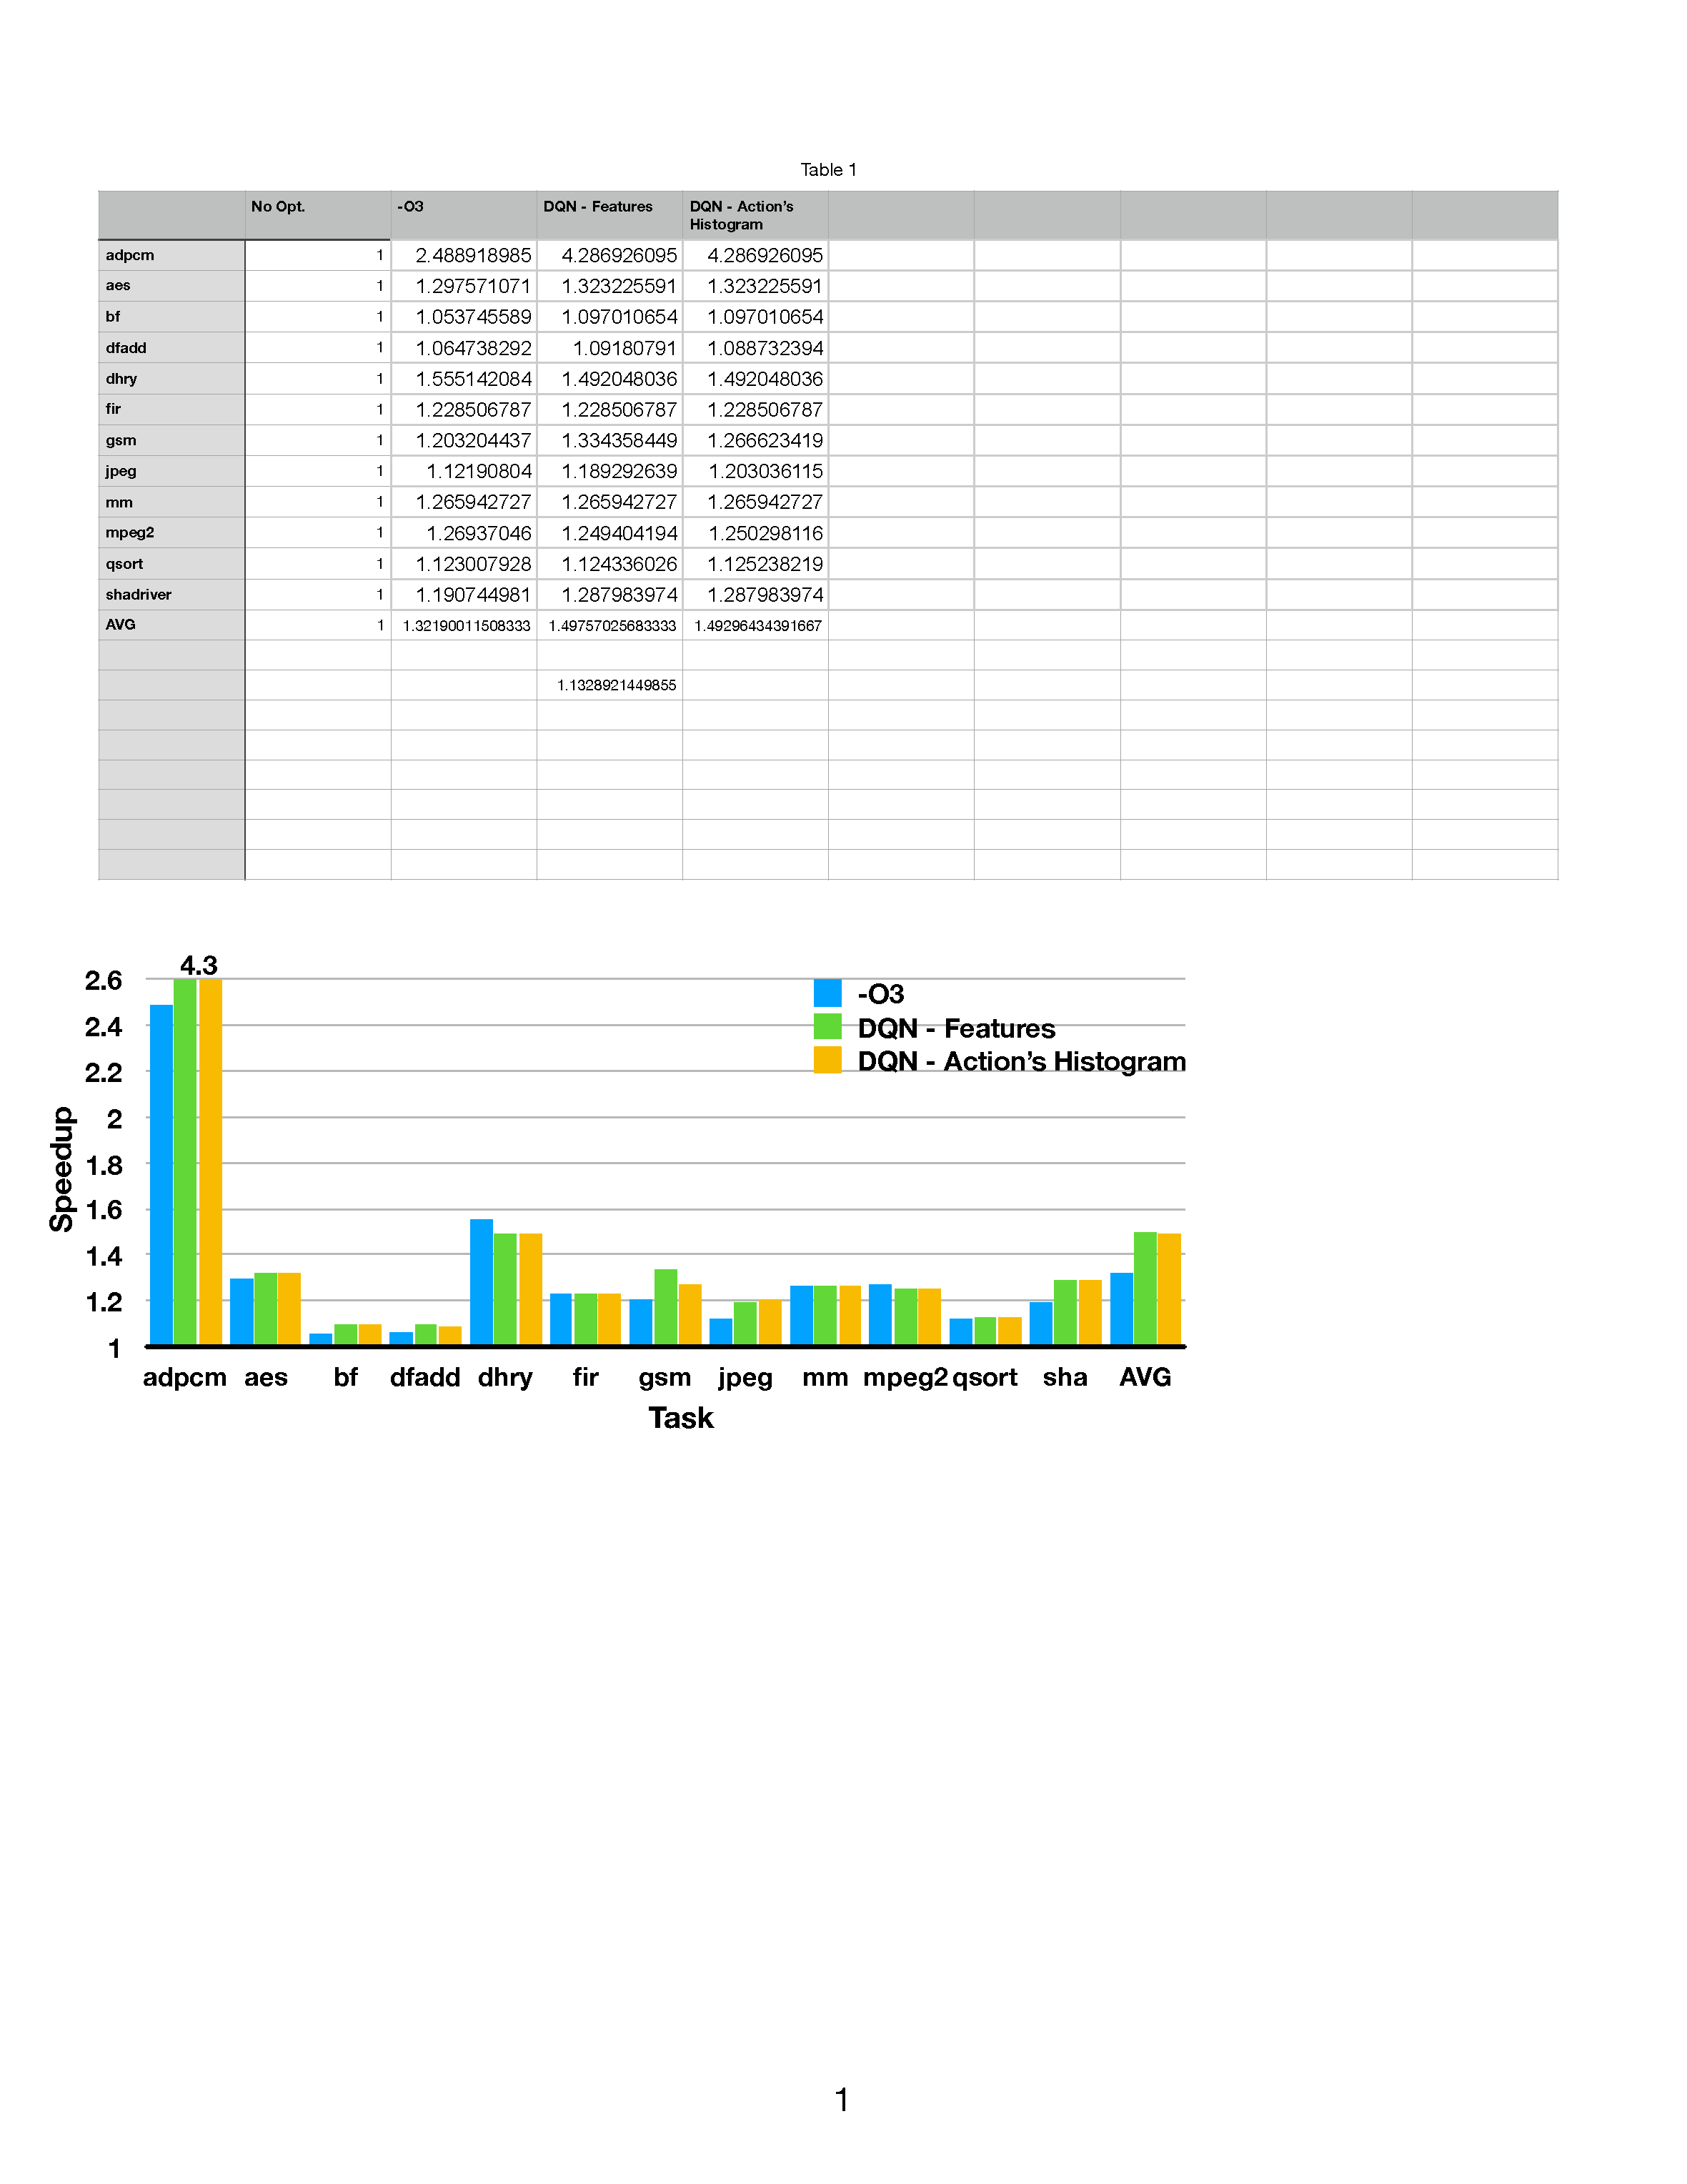
\includegraphics[trim={1.1cm 17.7cm 11.5cm 21.5cm},clip,width=0.5\textwidth]{Figures/model-action2.pdf} 
    \caption{The circuit speedup as function of algorithm training time for different optimization algorithms normalized to the performance without any optimization. The RL framework ran for 30 minutes on each program. \vspace*{-0.6cm}}
    \label{fig:model-action}
\end{figure}
\begin{figure}[!t]
    \centering
    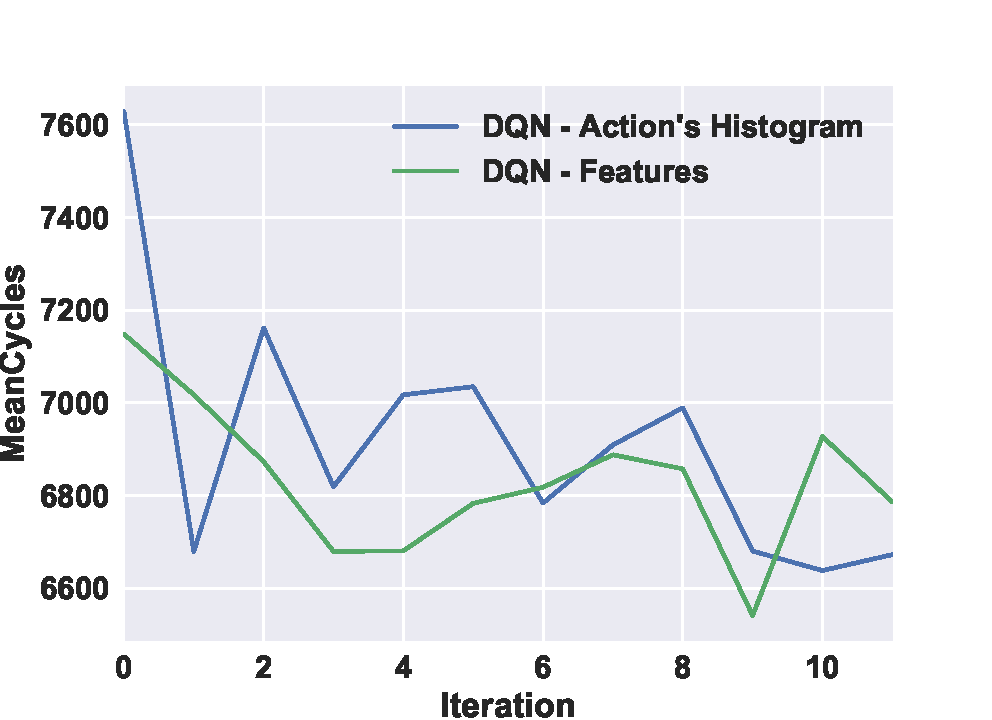
\includegraphics[trim={0cm 0cm 0cm 1cm},clip,width=0.5\textwidth]{Figures/gsm_model_action2.pdf}
    \vspace{-0.5cm}
    \caption{The mean cycles as function of time when running the framework on the gsm task. \vspace*{-0.6cm}}
    \label{fig:gsm_model_action}
\end{figure}

While both program feature and histogram approaches are efficient for operating on a single program, the histogram approach provided better performance in the long run. We observed that several passes are effective only if preceded by other passes, which may not change the program features significantly. For example, a pass may change only the order of instructions, but not their distribution. The network mistakenly learns to apply these effective passes directly and gain a zero benefit, resulting in unstable behavior. Furthermore, the space of features for various programs is sufficiently complex that it is difficult for a simple framework to learn, and it is not possible to derive a perfect optimization ordering on multiple programs simultaneously since each program has different features.

In contrast, using previous actions as the observation guarantees that after applying each pass the observation changes, making it less ambiguous for the network to learn. In addition, it enables operating on multiple programs simultaneously since the observation is independent from the program, which provides faster training. To further optimize the time it takes to run the framework we could also leverage the fact that the observations are directly extracted from the actions. This makes it possible to roll out an entire trajectory of actions and observations from the policy without compiling the programs. Effectively, we apply a pass, generate the new histogram, feed the new histogram to the policy again, which outputs a new pass and so on. The only things missing in this technique are the intermediate rewards that could be calculated by compiling the program after applying each pass, which we are trying to avoid as it takes a long time. 

In PG, the term in Equation~\ref{eq:policygradient} that depends on the reward value is the sum of rewards in the entire trajectory. This value could be obtained directly by compiling the program once at the end with all the applied passes. This makes using PG feasible although it generally requires more data samples and time to learn compared to DQN. In addition, in DQN, we could %compile once and average the reward for the labels in Equation~\ref{eq:Dqn} or 
compile a few times, each one after applying a sequence of actions and average the reward for all these actions. Beyond significantly reducing the training time, this approach helps alleviate the sparsity of rewards in cases where multiple passes are necessary to get a single reward and make the seemingly ineffective passes more effective. 


To operate on multiple programs simultaneously, the reward function was defined as follows:
\begin{multline}
     -reward_t = \sqrt[\leftroot{-2}\uproot{2}n]{C\_Prog_1(t) \cdot ... \cdot C\_Prog_n(t)} -
    \\
    \sqrt[\leftroot{-2}\uproot{2}n]{C\_Prog_1(t-1) \cdot ... \cdot C\_Prog_n(t-1)},
\end{multline}
where $n$ is the number of programs and $C\_Prog_i(t)$ is the cycle count of program $i$ at time step $t$. This reward function was chosen to guarantee that all programs are equally optimized; any improvement in one will positively affect the reward and make the rewards more dense. To speed the training process we took a multithreaded approach inspired by~\cite{mnih2016}. We implemented a multithreaded program that compiles the different programs simultaneously taking the same actions (passes) in each program.


%Note that the DQN and PG versions used in this work are in their simplest form and there are many improvements that mainly aim to reduce variance~\cite{van2016,Baxter2001}. Since our ultimate goal is to find a single trajectory that achieves the maximum reward and given that we want to find it as fast as possible, we can tradeoff this variance. %The performance of DQN could also be improved by using Double DQN (DDQN)~\cite{van2016}, which was used in the implemented framework.


 
% The most straightforward way to convert a program into an observation is achieved by extracting all the features of the program, \textit{i.e.} number of every operation as proposed by Wang \textit{et al.}~\cite{wang2018}. The features we extracted from the compiled programs are listed in Table \ref{tab:tab1} in the appendix. Nevertheless, these features proved to be not useful even after rigorous efforts on multiple RL algorithms, network configurations, which include fully connected (FC) networks, recurrent neural network~\cite{HausknechtS2015drl} and numerous network parameters search. We observed that several effective passes are effective only if preceded by other passes, which unfortunately do not change the observation. For example, if the pass only changes the order of instructions but not their distribution. The network mistakenly learns to apply these effective passes directly and gain a zero reward. %The issue is illustrated in Figure~\ref{fig:problem1}. 
% Furthermore, the space of features for various programs is too large and complicated to learn in a simple framework and it is not possible to learn on multiple programs simultaneously since each program has different features.
% \begin{figure}
%     \centering
%     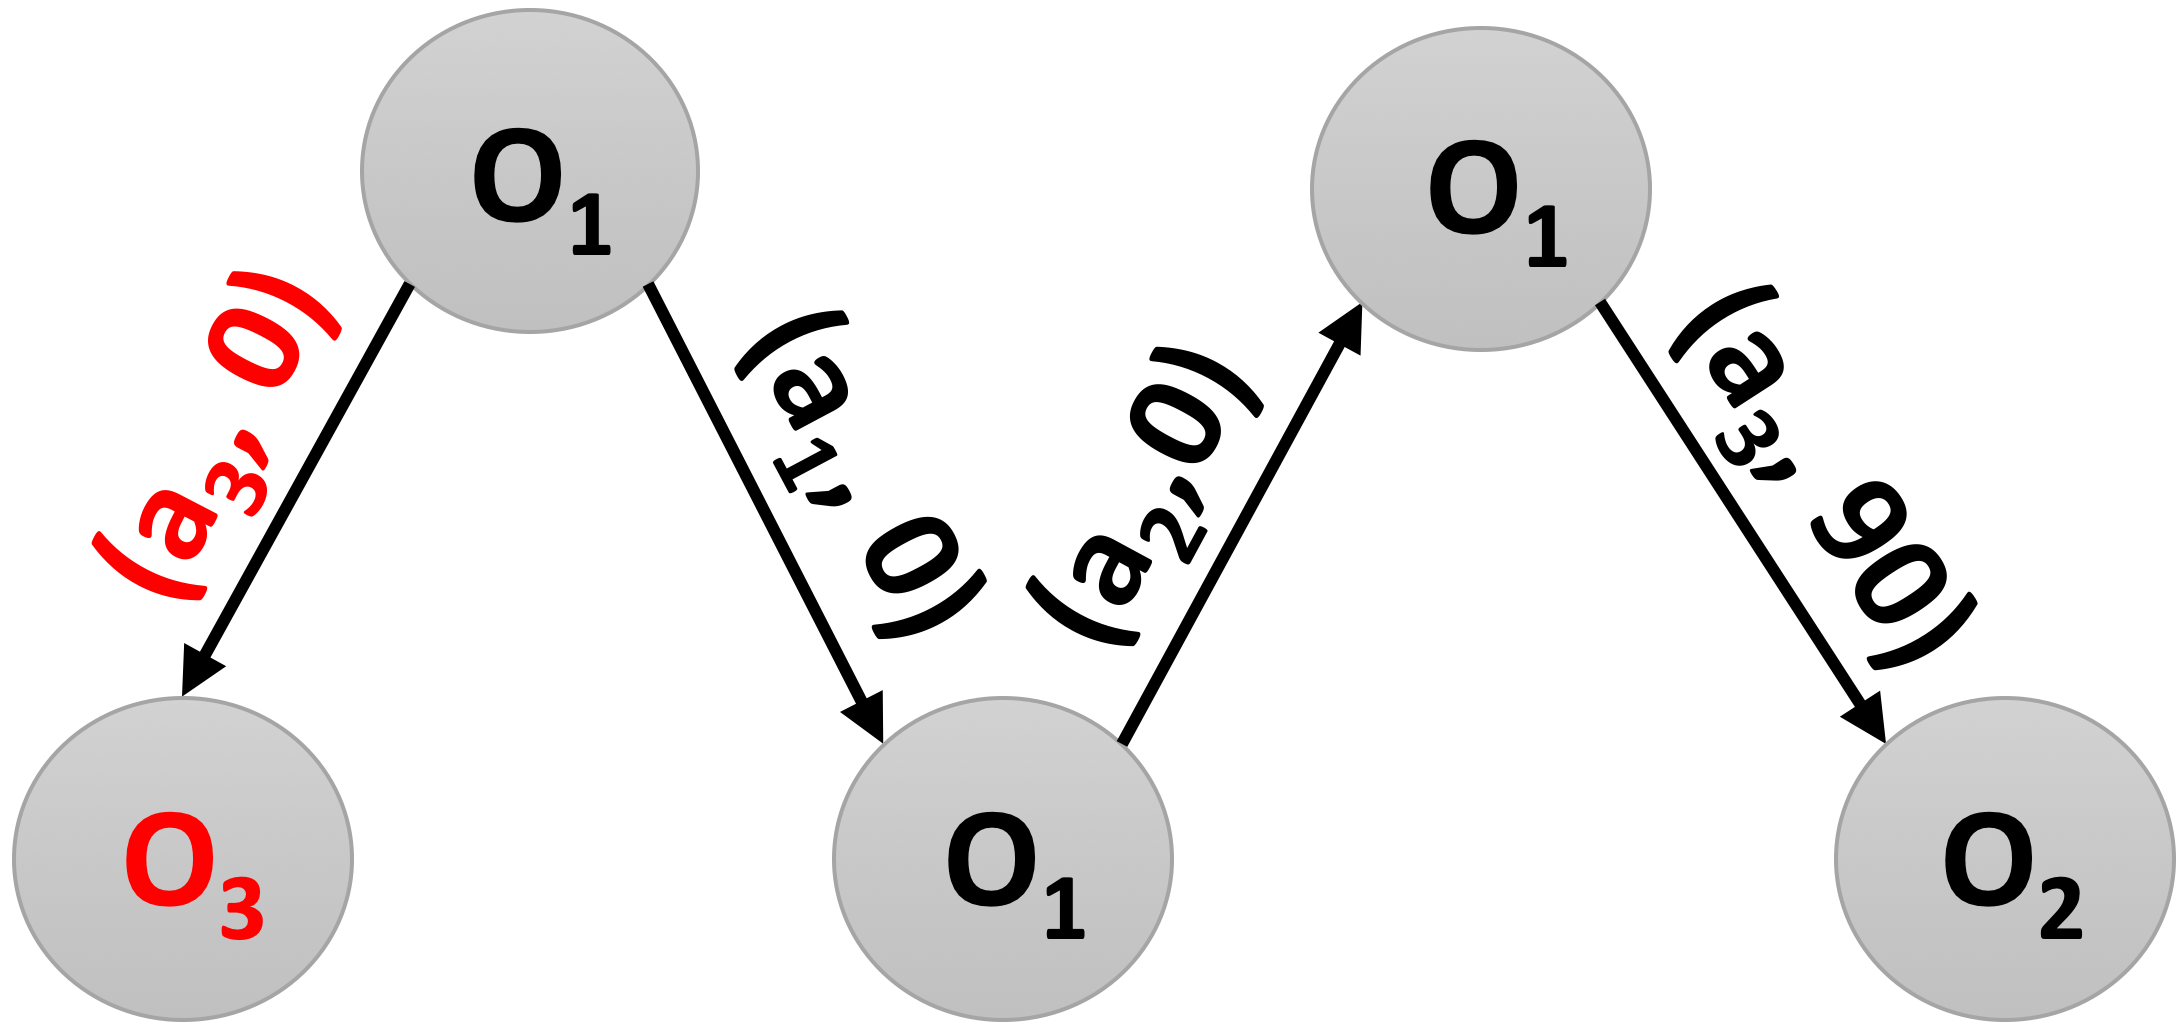
\includegraphics[width=0.45\textwidth]{Figures/problem.png}
%     \caption{The issue with using the number of different operations as observations. In order to achieve a reward of 90 the actions $a_1$ $\rightarrow$ $a_2$ $\rightarrow$ $a_3$ should be taken. But since the intermediate observations are similar and the intermediate rewards are 0, the network learns to apply $a_3$ directly and that $a_1$ and $a_2$ are ineffective. However, applying $a_3$ directly (as shown in red color) gives a reward of 0 and arrives at a different observation.}
%     \label{fig:problem1}
% \end{figure}


% To guarantee the observations change after applying each pass, and to enable operating on multiple programs simultaneously for efficiency, the actions were simply used as observations. In other words, the input of the network (observation) was defined as a histogram of the passes given so far and the passes were given an index from 0 to the number of passes. The output is the next pass to apply. This way the network can keep track of the passes given so far and learn which sequences should be applied to maximize the reward.


%(for example, in Figure~\ref{fig:problem1}, the actions $a_1$ and $a_2$ are effective but the network is blind to that because they contribute a zero reward). %The final algorithm is illustrated in figure~\ref{}.

\subsection{One-Hot Versus Histogram Representation}
% \begin{figure}
%     \centering
%     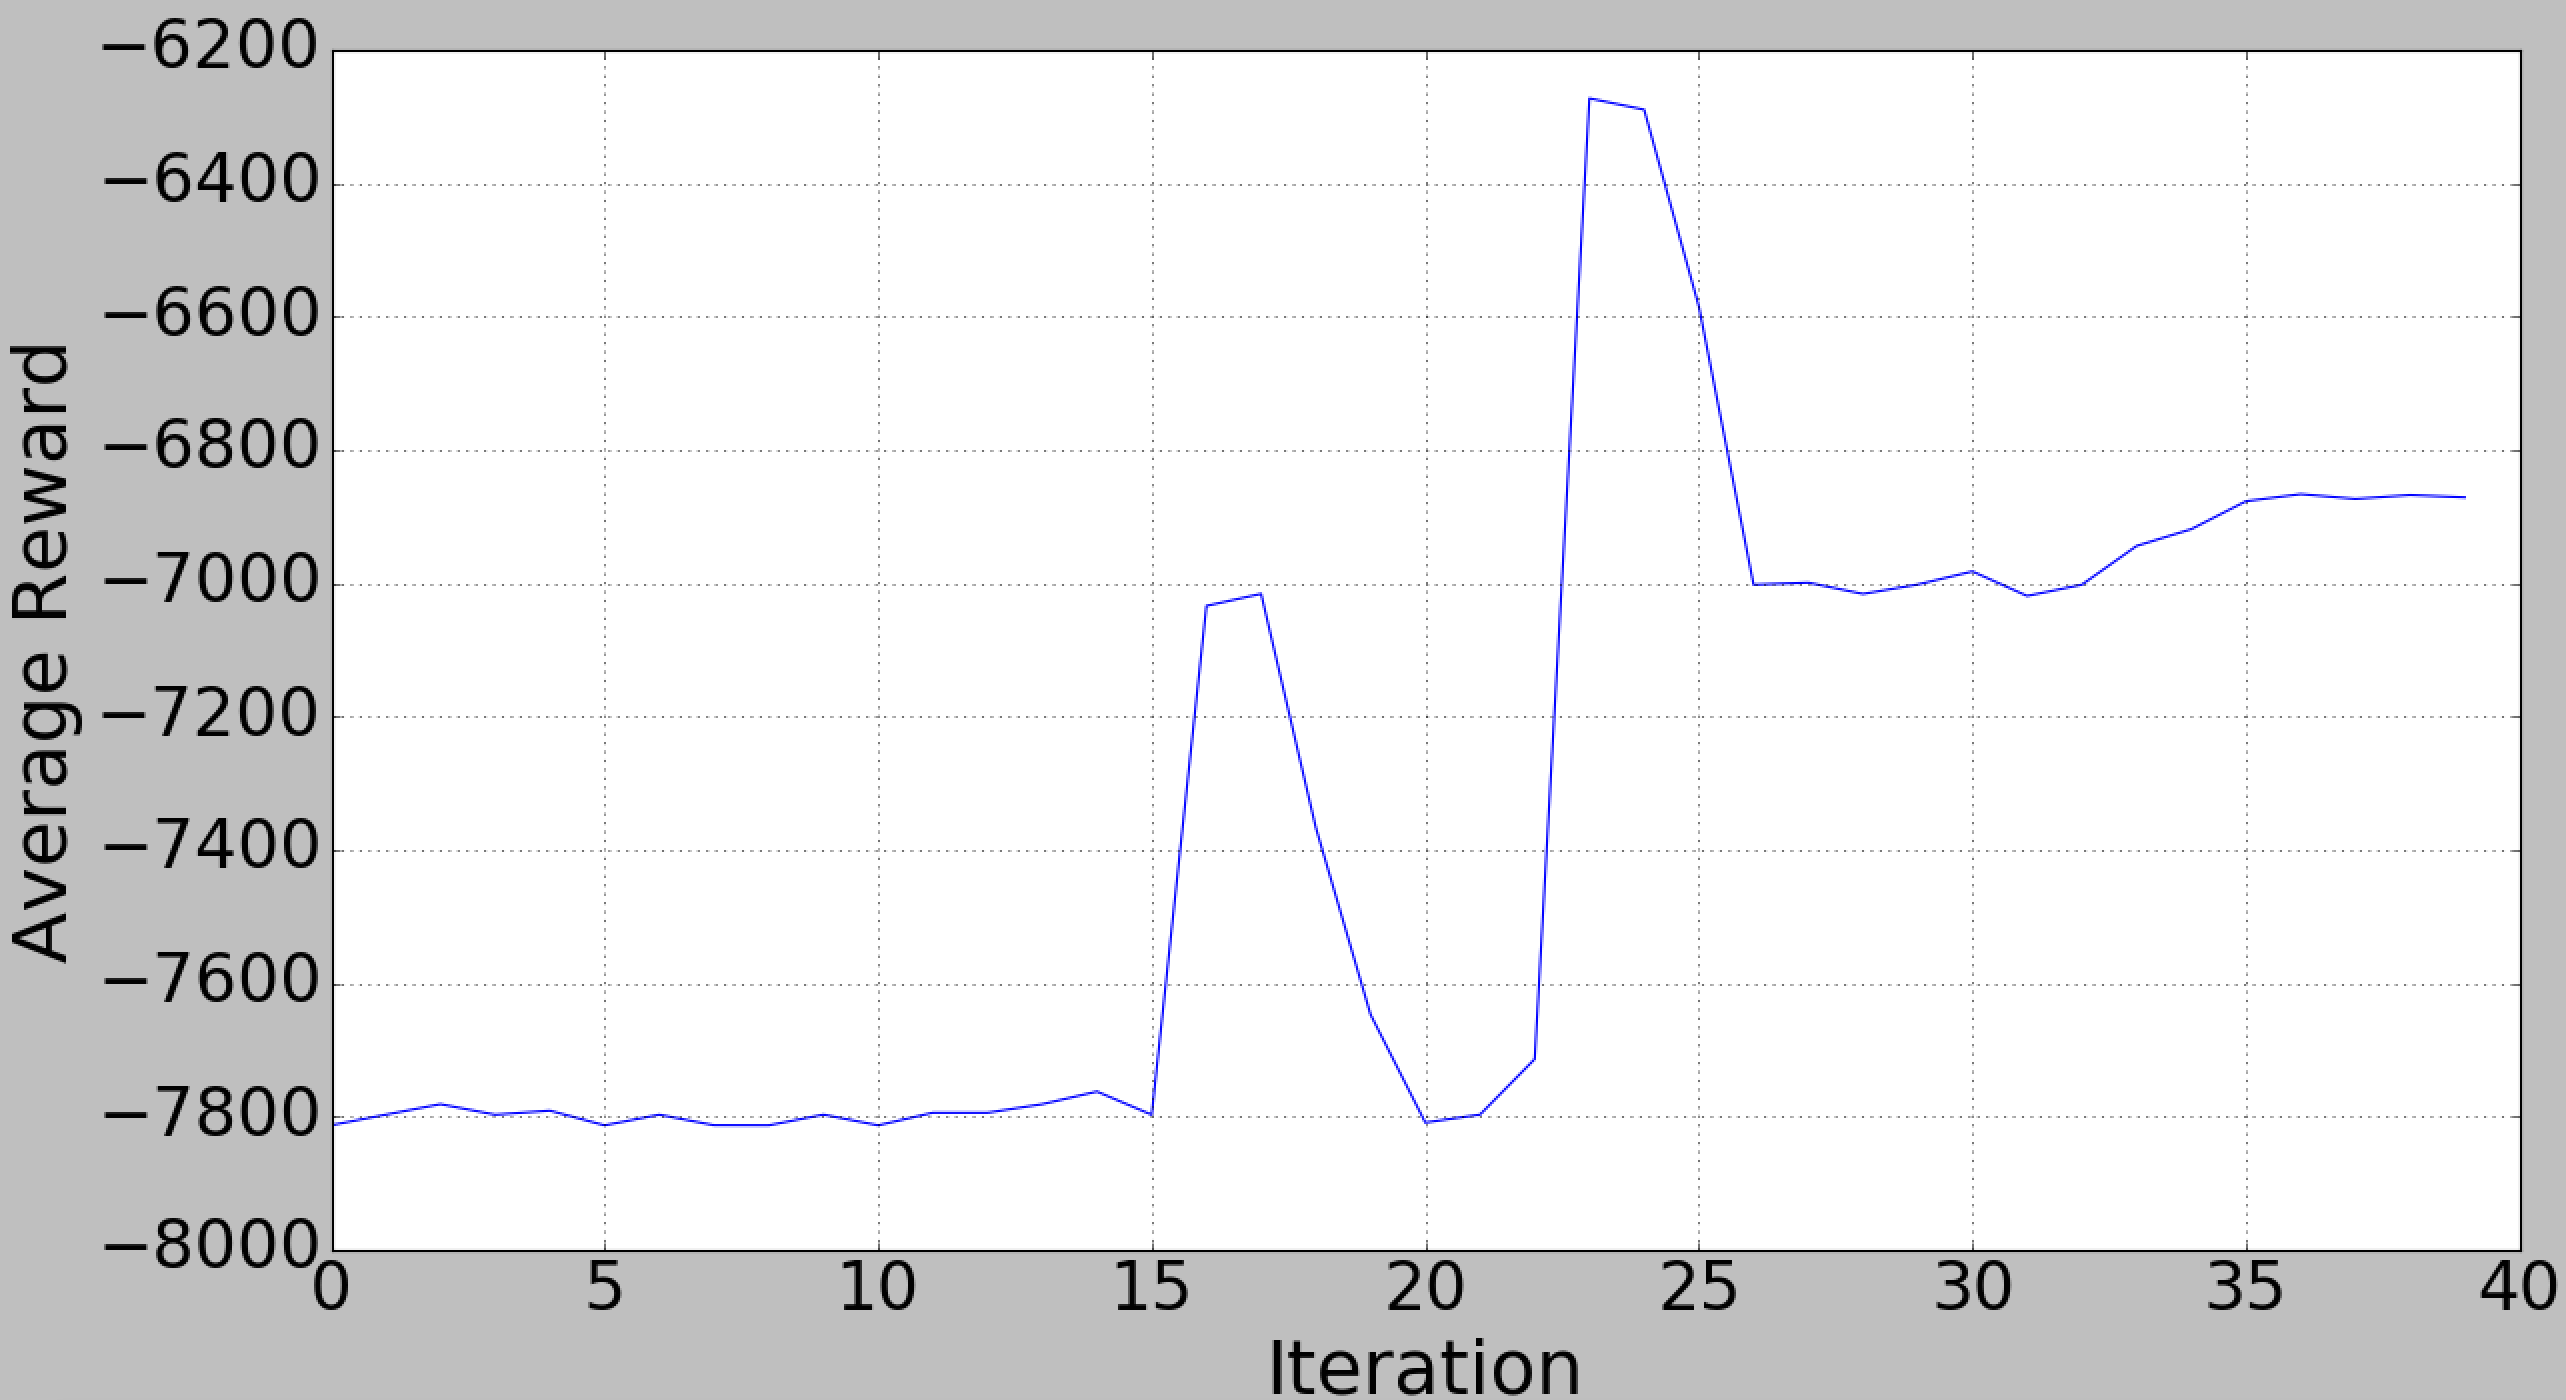
\includegraphics[width=0.5\textwidth]{Figures/gsmonlyhotone.png}    
%     \caption{The average reward (averaged over 50 steps) as a function of iteration for the gsm task. The maximum number of passes applied is five. The maximum reward achieved by the network is the global maximum possible with five passes.}
%     \label{fig:hotone}
% \end{figure}
% \begin{figure*}[!t]
%     \centering        
%     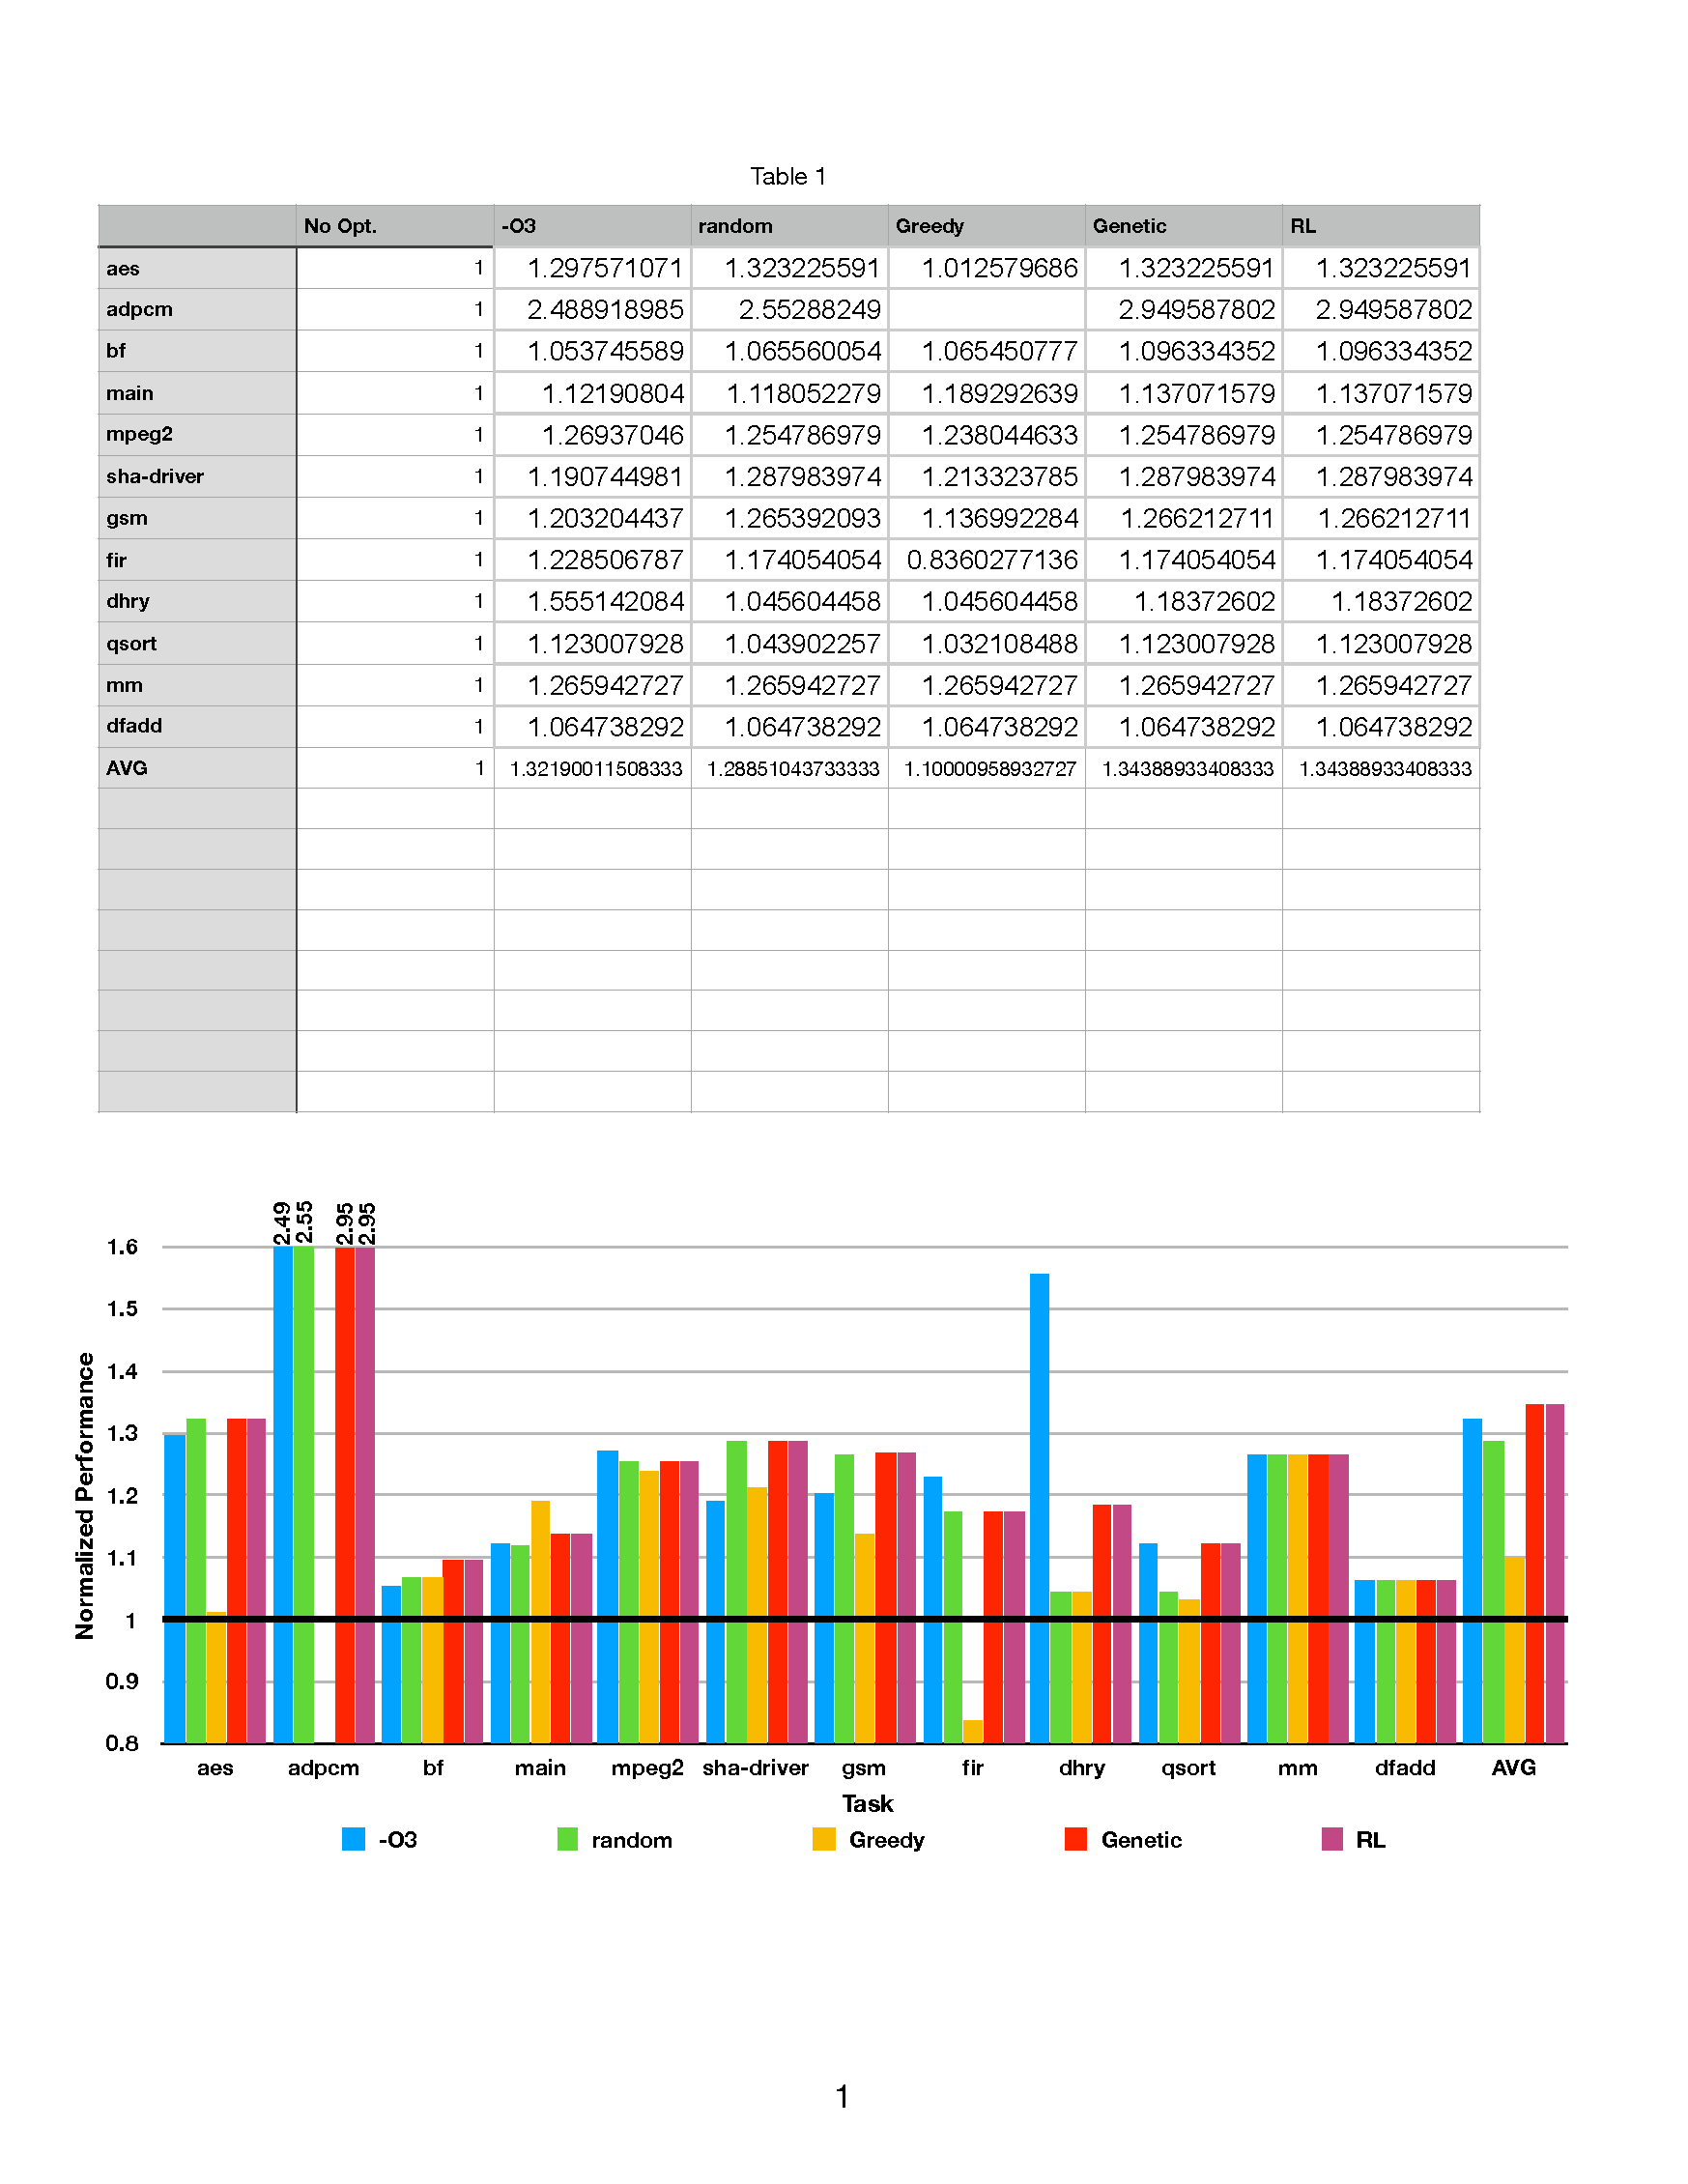
\includegraphics[trim={1.2cm 5.6cm 2cm 21cm},clip,width=\textwidth]{Figures/3passesv3.pdf} 
%     \caption{The performance for searching the best three passes using the different search algorithms for different tasks normalized to the case without any optimization. The exact number of cycles are listed in the appendix in Table~\ref{tab:3pass}}
%     \label{fig:3pass}
% \end{figure*}
Instead of using a histogram, a concatenation of $K$ one-hot vectors could be used, where $K$ is the number of passes to apply. The index $i$ of each vector$_j$ is $1$ if the $j^{th}$ pass applied is $i$, otherwise zero. This would allow RL to better understand the ordering of previously applied passes.
%The reward, for the hot one approach, on the gsm task, as a function of time step (averaged over 50 steps) is shown in Figure~\ref{fig:hotone}. The maximum number of passes applied is five. The network achieves the global maximum possible with five passes but it does not stabilize there. This could be due to the instability of DQN, network parameters, seeds, and large size of the network input observation. 
In practice, this did not improve performance largely because the state space is much larger, it takes a long time to learn. Moreover, increasing the maximum number of passes will make it effectively impossible for the network to learn. This is because adding one more pass requires adding $45$ inputs/features to the network (the total number of passes) making it more difficult for the network to converge.